\section{Methodology}
\label{sec-methodology}

%Describe your approach and design
%Instead of simply explaining what you ended up doing, show why you made such
%design decisions / how what the trade-offs are.

As mentioned earlier, DRAM power consumption is dominated by
charging/discharging chip capacitances and signal reflections caused by link
terminations. Once the capacitors have reached steady state, their power
consumption is negligible in comparison to the system as a whole and thus can
be neglected from our power models. Instead we focus on link termination and
signal reflections. Specifically, DDR4 memory technology leverages \TT{DBI} to
reduce the signal reflections and power consumption. Intuitively, DBI aims to
reduce the number of bit flips (DBI-AC) and binary signal probabilities
(DBI-DC) to improve power consumption of read and write operations. For
reducing bit flips, take for example the case where memory location $M$
previously had the value $00000000$ that was being overwritten by the value
$11111111$. Instead of flipping every bit in $M$, a DBI-AC enabled memory system
would retain the previos state of $00000000$ and set the DBI flag that
signifies that all the bits are flipped.  This would incur the power conumption
of 1 bit flip, not the entire data byte.  Since the power consumption of 0 and
1 is not the same, depending on memory technology constraints, DBI-DC aims to
reduce the prevalance of the higher power consuming bit. In the case of DDR4,
$0$ consumes more power and thus DBI aims to reduce the number of $0$'s and
increase the number of $1$'s \fixme{add citation}. Figure \ref{fig:dbi-dc}
illustrates the impact of DBI-DC on improving signal quality and consequently
power consumption of read and write operations. The larger open data eye
illustrates that there is less interference between the driver and reflected
signals when using DBI-DC and the samller $V_{pp}$ suggests that the driver has
to work less with DBI-DC enabled.

\begin{figure}[!htb]
  \centering
  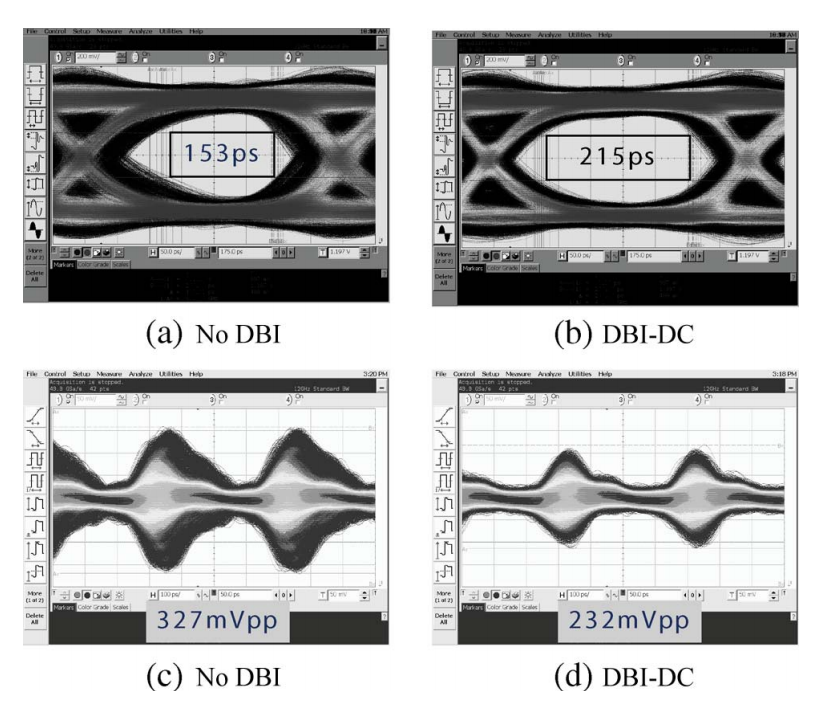
\includegraphics[width=0.3\textwidth]{figs/dbi-dc}
  \caption{DBI DC Impact \cite{hollis}}
  \label{fig:dbi-dc}
\end{figure}

\subsection{Model}


\begin{enumerate}
  \item Introduce equation
    $$ P_t = A \times P_{dc} + B \times P_{ac}$$
  \item Talk about encrypted data : A = 0.5, B = 0.5 : Assumption that Data is
    Completely random once encrypted
  \item Say that DBI aims to reduce A, B by using program structure
\end{enumerate}

\subsection{Experimental Setup}
\begin{enumerate}
  \item PIN - dynamic binary instrumentaiton tool : describe cache settings
  \item Computer architecture analysis tool
  \item MiBench - Justify why MiBench (mobile) ---- SPEC is not as good
  \item DRAMSim - Did not work for us.
  \item Python Script to analyze the loads and stores from the trace outptted
    from PIN
\end{enumerate}
